% Standalone TikZ figure: Domain Randomization Parameter Taxonomy
% For Chapter 4: Synthetic Data Generation for Object Detection
\documentclass[tikz,border=10pt]{standalone}
\usepackage{tikz}
\usetikzlibrary{arrows.meta, positioning, shapes.geometric, fit, backgrounds, calc, trees}

\begin{document}
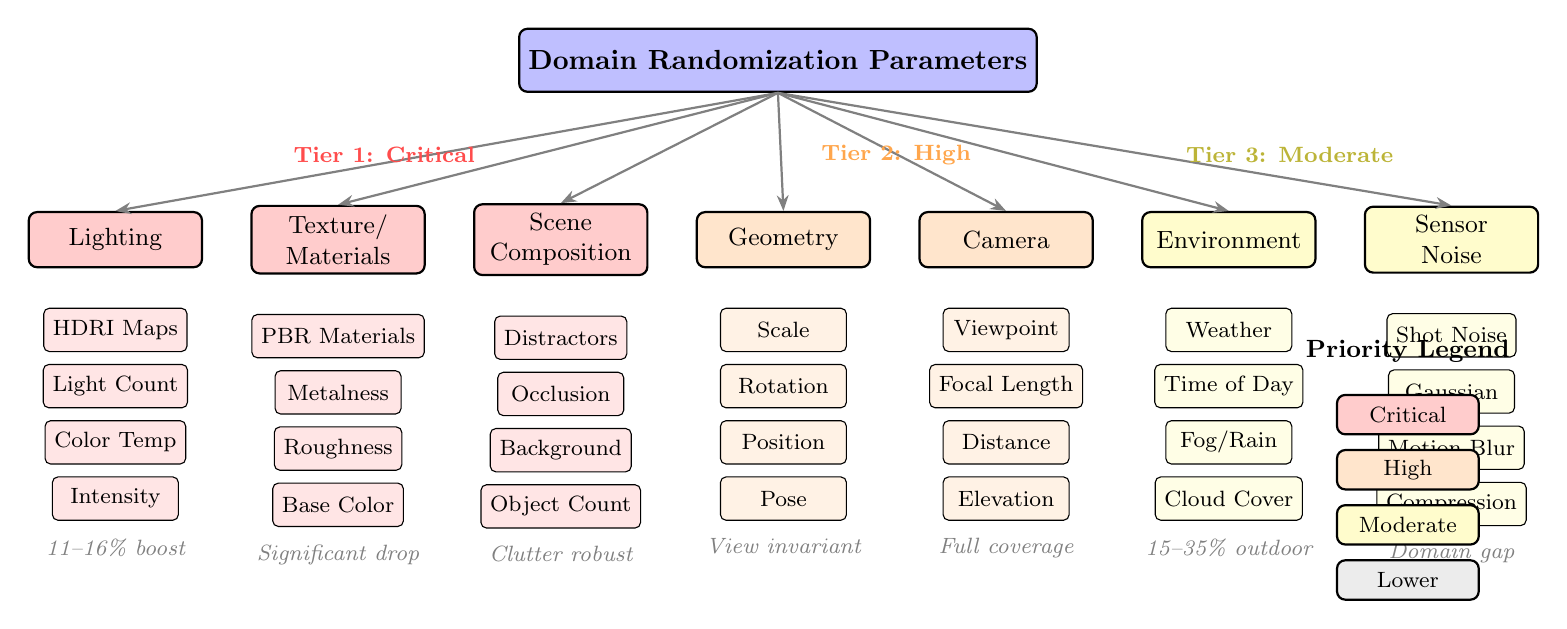
\begin{tikzpicture}[
    every node/.style={font=\small},
    level 1/.style={sibling distance=3.2cm, level distance=1.8cm},
    level 2/.style={sibling distance=1.4cm, level distance=1.5cm},
    root/.style={rectangle, draw, thick, fill=blue!25, minimum width=3cm, minimum height=0.8cm, rounded corners=3pt, font=\bfseries},
    cat/.style={rectangle, draw, thick, minimum width=2.2cm, minimum height=0.7cm, rounded corners=3pt, align=center},
    param/.style={rectangle, draw, minimum width=1.6cm, minimum height=0.55cm, rounded corners=2pt, align=center, font=\footnotesize},
    tier1/.style={cat, fill=red!20},
    tier2/.style={cat, fill=orange!20},
    tier3/.style={cat, fill=yellow!20},
    tier4/.style={cat, fill=gray!15},
    arrow/.style={-{Stealth[length=2mm]}, thick}
]

% Root node
\node[root] (root) {Domain Randomization Parameters};

% Tier 1 - Critical Impact (left side)
\node[tier1, below left=1.5cm and 4cm of root] (light) {Lighting};
\node[tier1, right=0.6cm of light] (texture) {Texture/\\Materials};
\node[tier1, right=0.6cm of texture] (scene) {Scene\\Composition};

% Tier 2 - High Impact
\node[tier2, right=0.6cm of scene] (geom) {Geometry};
\node[tier2, right=0.6cm of geom] (camera) {Camera};

% Tier 3 - Moderate Impact
\node[tier3, right=0.6cm of camera] (environ) {Environment};
\node[tier3, right=0.6cm of environ] (noise) {Sensor\\Noise};

% Connections from root
\foreach \n in {light, texture, scene, geom, camera, environ, noise} {
    \draw[arrow, gray] (root.south) -- (\n.north);
}

% Lighting parameters
\node[param, fill=red!10, below=0.5cm of light] (l1) {HDRI Maps};
\node[param, fill=red!10, below=0.15cm of l1] (l2) {Light Count};
\node[param, fill=red!10, below=0.15cm of l2] (l3) {Color Temp};
\node[param, fill=red!10, below=0.15cm of l3] (l4) {Intensity};

% Texture parameters
\node[param, fill=red!10, below=0.5cm of texture] (t1) {PBR Materials};
\node[param, fill=red!10, below=0.15cm of t1] (t2) {Metalness};
\node[param, fill=red!10, below=0.15cm of t2] (t3) {Roughness};
\node[param, fill=red!10, below=0.15cm of t3] (t4) {Base Color};

% Scene composition parameters
\node[param, fill=red!10, below=0.5cm of scene] (s1) {Distractors};
\node[param, fill=red!10, below=0.15cm of s1] (s2) {Occlusion};
\node[param, fill=red!10, below=0.15cm of s2] (s3) {Background};
\node[param, fill=red!10, below=0.15cm of s3] (s4) {Object Count};

% Geometry parameters
\node[param, fill=orange!10, below=0.5cm of geom] (g1) {Scale};
\node[param, fill=orange!10, below=0.15cm of g1] (g2) {Rotation};
\node[param, fill=orange!10, below=0.15cm of g2] (g3) {Position};
\node[param, fill=orange!10, below=0.15cm of g3] (g4) {Pose};

% Camera parameters
\node[param, fill=orange!10, below=0.5cm of camera] (c1) {Viewpoint};
\node[param, fill=orange!10, below=0.15cm of c1] (c2) {Focal Length};
\node[param, fill=orange!10, below=0.15cm of c2] (c3) {Distance};
\node[param, fill=orange!10, below=0.15cm of c3] (c4) {Elevation};

% Environment parameters
\node[param, fill=yellow!10, below=0.5cm of environ] (e1) {Weather};
\node[param, fill=yellow!10, below=0.15cm of e1] (e2) {Time of Day};
\node[param, fill=yellow!10, below=0.15cm of e2] (e3) {Fog/Rain};
\node[param, fill=yellow!10, below=0.15cm of e3] (e4) {Cloud Cover};

% Noise parameters
\node[param, fill=yellow!10, below=0.5cm of noise] (n1) {Shot Noise};
\node[param, fill=yellow!10, below=0.15cm of n1] (n2) {Gaussian};
\node[param, fill=yellow!10, below=0.15cm of n2] (n3) {Motion Blur};
\node[param, fill=yellow!10, below=0.15cm of n3] (n4) {Compression};

% Tier labels
\node[font=\footnotesize\bfseries, text=red!70] at (-5, -1.2) {Tier 1: Critical};
\node[font=\footnotesize\bfseries, text=orange!70] at (1.5, -1.2) {Tier 2: High};
\node[font=\footnotesize\bfseries, text=yellow!70!black] at (6.5, -1.2) {Tier 3: Moderate};

% Impact annotations
\node[font=\footnotesize\itshape, text=gray, below=0.1cm of l4] {11--16\% boost};
\node[font=\footnotesize\itshape, text=gray, below=0.1cm of t4] {Significant drop};
\node[font=\footnotesize\itshape, text=gray, below=0.1cm of s4] {Clutter robust};
\node[font=\footnotesize\itshape, text=gray, below=0.1cm of g4] {View invariant};
\node[font=\footnotesize\itshape, text=gray, below=0.1cm of c4] {Full coverage};
\node[font=\footnotesize\itshape, text=gray, below=0.1cm of e4] {15--35\% outdoor};
\node[font=\footnotesize\itshape, text=gray, below=0.1cm of n4] {Domain gap};

% Legend
\begin{scope}[shift={(8,-4.5)}]
    \node[font=\bfseries\small] at (0, 0.8) {Priority Legend};
    \node[tier1, minimum width=1.8cm, minimum height=0.5cm] at (0, 0) {};
    \node[font=\footnotesize] at (0, 0) {Critical};
    \node[tier2, minimum width=1.8cm, minimum height=0.5cm] at (0, -0.7) {};
    \node[font=\footnotesize] at (0, -0.7) {High};
    \node[tier3, minimum width=1.8cm, minimum height=0.5cm] at (0, -1.4) {};
    \node[font=\footnotesize] at (0, -1.4) {Moderate};
    \node[tier4, minimum width=1.8cm, minimum height=0.5cm] at (0, -2.1) {};
    \node[font=\footnotesize] at (0, -2.1) {Lower};
\end{scope}

\end{tikzpicture}
\end{document}
